\chapter{Additional tables and plot from Chapter~\ref{reflectometry1}}

\ref{refl1app}

%
\begin{table}
    \centering
    \small
    \caption{The best-fit values, and associated \SI{95}{\percent} confidence intervals for each of the varying parameters for each phospholipid at the lowest surface pressure measured from XRR. The values of $\phi_h$ were obtained from the appropriate use of Equation~\protect\ref{equ:phih}.}
    \label{tab:xrrref1}
    \begin{tabular}{l | l l l l}
        \toprule
        Phospholipid & DPPC & DMPC & DLPC & DMPG \\
        Surface Pressure/\si{\milli\newton\per\meter} & 15 & 20 & 20 & 15 \\
        \midrule
        $V_t$/\si{\angstrom\cubed} & \input{output/reflectometry1/dppc_xray/dppc_xray-V_t} & \input{output/reflectometry1/dmpc_xray/dmpc_xray-V_t} & \input{output/reflectometry1/dlpc_xray/dlpc_xray-V_t} & \input{output/reflectometry1/dmpg_xray/dmpg_xray-V_t} \\
        $V_h$/\si{\angstrom\cubed} & \input{output/reflectometry1/dppc_xray/dppc_xray-V_h} & \input{output/reflectometry1/dmpc_xray/dmpc_xray-V_h} & \input{output/reflectometry1/dlpc_xray/dlpc_xray-V_h} & \input{output/reflectometry1/dmpg_xray/dmpg_xray-V_h} \\
        $d_h$/\si{\angstrom} & \input{output/reflectometry1/dppc_xray/dppc_xray-d_h} & \input{output/reflectometry1/dmpc_xray/dmpc_xray-d_h} & \input{output/reflectometry1/dlpc_xray/dlpc_xray-d_h} & \input{output/reflectometry1/dmpg_xray/dmpg_xray-d_h} \\
        \midrule
        $d_t$\si{\angstrom} & \input{output/reflectometry1/dppc_xray/dppc_xray-d_t_15} & \input{output/reflectometry1/dmpc_xray/dmpc_xray-d_t_20} & \input{output/reflectometry1/dlpc_xray/dlpc_xray-d_t_20} & \input{output/reflectometry1/dmpg_xray/dmpg_xray-d_t_15} \\
        $\sigma_{t,h,s}$/\si{\angstrom} & \input{output/reflectometry1/dppc_xray/dppc_xray_rough_15} & \input{output/reflectometry1/dmpc_xray/dmpc_xray_rough_20} & \input{output/reflectometry1/dlpc_xray/dlpc_xray_rough_20} & \input{output/reflectometry1/dmpg_xray/dmpg_xray_rough_15} \\
        \midrule
        $\phi_h$/$\times 10^{-2}$ & \input{output/reflectometry1/dppc_xray/dppc_xray-phih_15} & \input{output/reflectometry1/dmpc_xray/dmpc_xray-phih_20} & \input{output/reflectometry1/dlpc_xray/dlpc_xray-phih_20} & \input{output/reflectometry1/dmpg_xray/dmpg_xray-phih_15} \\
        \bottomrule
    \end{tabular}
\end{table}
%
%
\begin{table}
    \centering
    \small
    \caption{The best-fit values, and associated \SI{95}{\percent} confidence intervals for each of the varying parameters for each phospholipid at the second lowest surface pressure measured from XRR. The values of $\phi_h$ were obtained from the appropriate use of Equation~\protect\ref{equ:phih}.}
    \label{tab:xrrref2}
    \begin{tabular}{l | l l l l}
        \toprule
        Phospholipid & DPPC & DMPC & DLPC & DMPG \\
        Surface Pressure/\si{\milli\newton\per\meter} & 20 & 25 & 25 & 20 \\
        \midrule
        $V_t$/\si{\angstrom\cubed} & \input{output/reflectometry1/dppc_xray/dppc_xray-V_t} & \input{output/reflectometry1/dmpc_xray/dmpc_xray-V_t} & \input{output/reflectometry1/dlpc_xray/dlpc_xray-V_t} & \input{output/reflectometry1/dmpg_xray/dmpg_xray-V_t} \\
        $V_h$/\si{\angstrom\cubed} & \input{output/reflectometry1/dppc_xray/dppc_xray-V_h} & \input{output/reflectometry1/dmpc_xray/dmpc_xray-V_h} & \input{output/reflectometry1/dlpc_xray/dlpc_xray-V_h} & \input{output/reflectometry1/dmpg_xray/dmpg_xray-V_h} \\
        $d_h$/\si{\angstrom} & \input{output/reflectometry1/dppc_xray/dppc_xray-d_h} & \input{output/reflectometry1/dmpc_xray/dmpc_xray-d_h} & \input{output/reflectometry1/dlpc_xray/dlpc_xray-d_h} & \input{output/reflectometry1/dmpg_xray/dmpg_xray-d_h} \\
        \midrule
        $d_t$\si{\angstrom} & \input{output/reflectometry1/dppc_xray/dppc_xray-d_t_20} & \input{output/reflectometry1/dmpc_xray/dmpc_xray-d_t_25} & \input{output/reflectometry1/dlpc_xray/dlpc_xray-d_t_25} & \input{output/reflectometry1/dmpg_xray/dmpg_xray-d_t_20} \\
        $\sigma_{t,h,s}$/\si{\angstrom} & \input{output/reflectometry1/dppc_xray/dppc_xray_rough_20} & \input{output/reflectometry1/dmpc_xray/dmpc_xray_rough_25} & \input{output/reflectometry1/dlpc_xray/dlpc_xray_rough_25} & \input{output/reflectometry1/dmpg_xray/dmpg_xray_rough_20} \\
        \midrule
        $\phi_h$/$\times 10^{-2}$ & \input{output/reflectometry1/dppc_xray/dppc_xray-phih_20} & \input{output/reflectometry1/dmpc_xray/dmpc_xray-phih_25} & \input{output/reflectometry1/dlpc_xray/dlpc_xray-phih_25} & \input{output/reflectometry1/dmpg_xray/dmpg_xray-phih_20} \\
        \bottomrule
    \end{tabular}
\end{table}
%
%
\begin{table}
    \centering
    \small
    \caption{The best-fit values, and associated \SI{95}{\percent} confidence intervals for each of the varying parameters for each phospholipid at the highest surface pressure measured from XRR. The values of $\phi_h$ were obtained from the appropriate use of Equation~\protect\ref{equ:phih}.}
    \label{tab:xrrref4}
    \begin{tabular}{l | l l l l}
        \toprule
        Phospholipid & DPPC & DMPC & DLPC & DMPG \\
        Surface Pressure/\si{\milli\newton\per\meter} & 30 & 40 & 35 & 30 \\
        \midrule
        $V_t$/\si{\angstrom\cubed} & \input{output/reflectometry1/dppc_xray/dppc_xray-V_t} & \input{output/reflectometry1/dmpc_xray/dmpc_xray-V_t} & \input{output/reflectometry1/dlpc_xray/dlpc_xray-V_t} & \input{output/reflectometry1/dmpg_xray/dmpg_xray-V_t} \\
        $V_h$/\si{\angstrom\cubed} & \input{output/reflectometry1/dppc_xray/dppc_xray-V_h} & \input{output/reflectometry1/dmpc_xray/dmpc_xray-V_h} & \input{output/reflectometry1/dlpc_xray/dlpc_xray-V_h} & \input{output/reflectometry1/dmpg_xray/dmpg_xray-V_h} \\
        $d_h$/\si{\angstrom} & \input{output/reflectometry1/dppc_xray/dppc_xray-d_h} & \input{output/reflectometry1/dmpc_xray/dmpc_xray-d_h} & \input{output/reflectometry1/dlpc_xray/dlpc_xray-d_h} & \input{output/reflectometry1/dmpg_xray/dmpg_xray-d_h} \\
        \midrule
        $d_t$\si{\angstrom} & \input{output/reflectometry1/dppc_xray/dppc_xray-d_t_30} & \input{output/reflectometry1/dmpc_xray/dmpc_xray-d_t_40} & \input{output/reflectometry1/dlpc_xray/dlpc_xray-d_t_35} & \input{output/reflectometry1/dmpg_xray/dmpg_xray-d_t_30} \\
        $\sigma_{t,h,s}$/\si{\angstrom} & \input{output/reflectometry1/dppc_xray/dppc_xray_rough_30} & \input{output/reflectometry1/dmpc_xray/dmpc_xray_rough_40} & \input{output/reflectometry1/dlpc_xray/dlpc_xray_rough_35} & \input{output/reflectometry1/dmpg_xray/dmpg_xray_rough_30} \\
        \midrule
        $\phi_h$/$\times 10^{-2}$ & \input{output/reflectometry1/dppc_xray/dppc_xray-phih_30} & \input{output/reflectometry1/dmpc_xray/dmpc_xray-phih_40} & \input{output/reflectometry1/dlpc_xray/dlpc_xray-phih_35} & \input{output/reflectometry1/dmpg_xray/dmpg_xray-phih_30} \\
        \bottomrule
    \end{tabular}
\end{table}
%
%
\begin{figure}
    \centering
    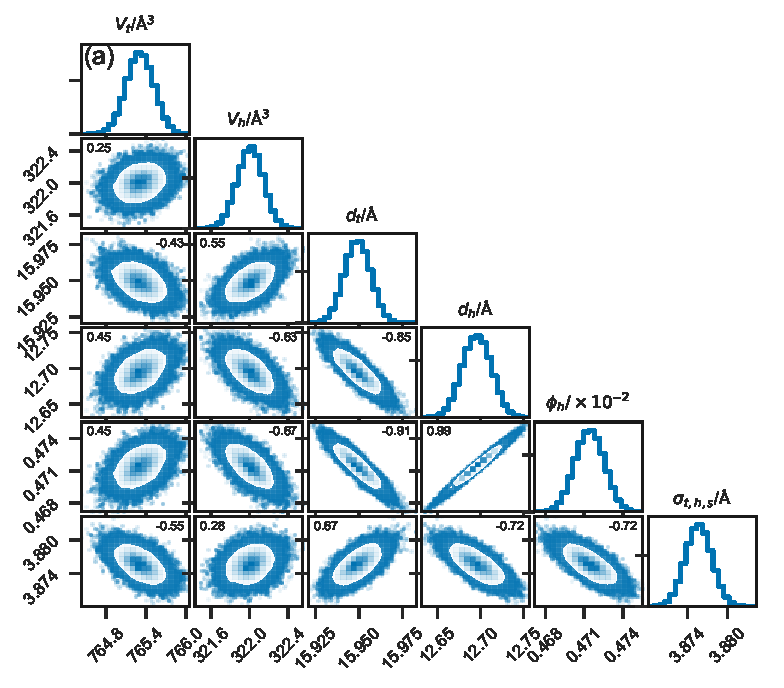
\includegraphics[width=0.49\textwidth]{reflectometry1/dppc_xray_sp_15_pdf}
    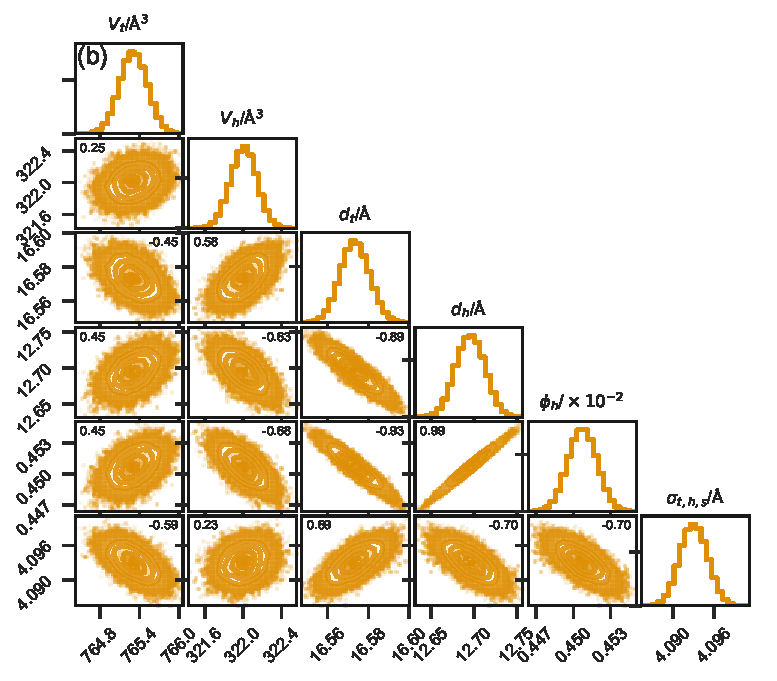
\includegraphics[width=0.49\textwidth]{reflectometry1/dppc_xray_sp_20_pdf} \\
    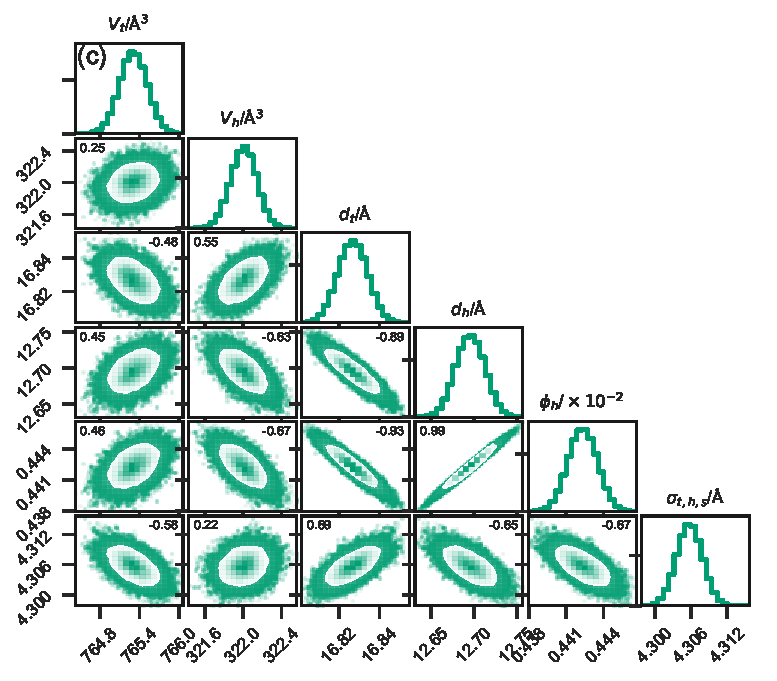
\includegraphics[width=0.49\textwidth]{reflectometry1/dppc_xray_sp_25_pdf}
    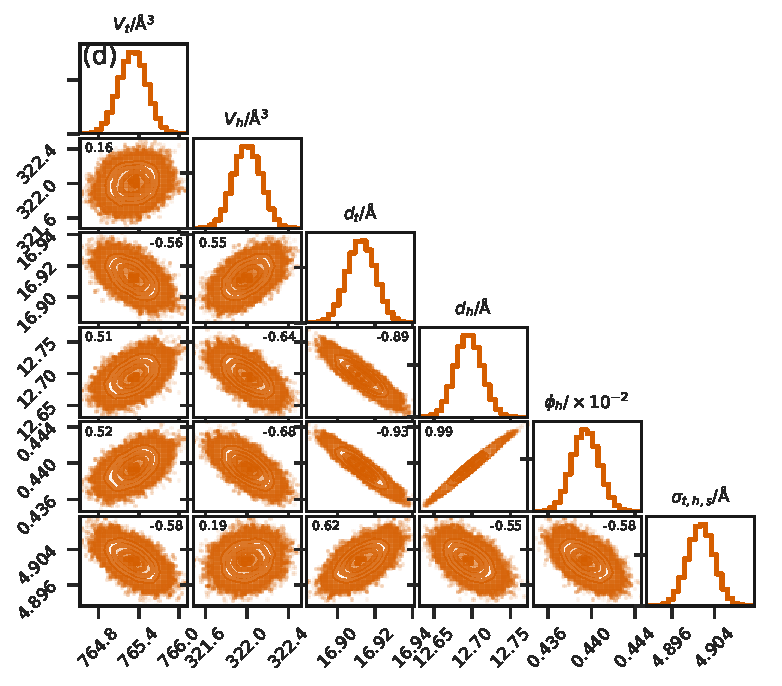
\includegraphics[width=0.49\textwidth]{reflectometry1/dppc_xray_sp_30_pdf}
    \caption{The probability distribution functions from the chemically-consistent modelling of DPPC; (a) at \SI{15}{\milli\newton\per\meter}, (b) at \SI{20}{\milli\newton\per\meter}, (c) at \SI{25}{\milli\newton\per\meter}, (d) at \SI{30}{\milli\newton\per\meter}. The Pearson correlation coefficient for each pair of parameters is given in the top corner of each two-dimensional PDF.}
    \label{fig:dppcpdfs}
\end{figure}
%
%
\begin{figure}
    \centering
    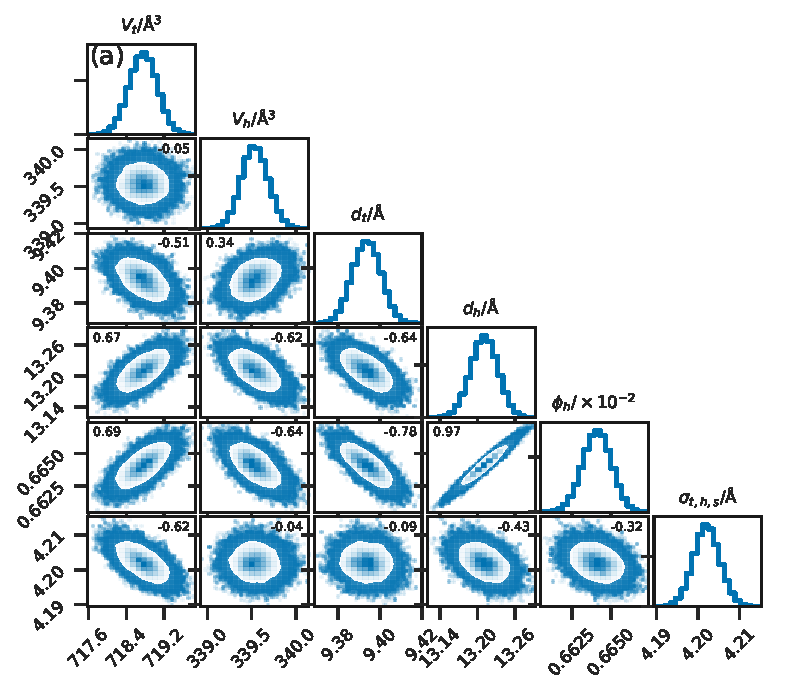
\includegraphics[width=0.49\textwidth]{reflectometry1/dmpc_xray_sp_20_pdf}
    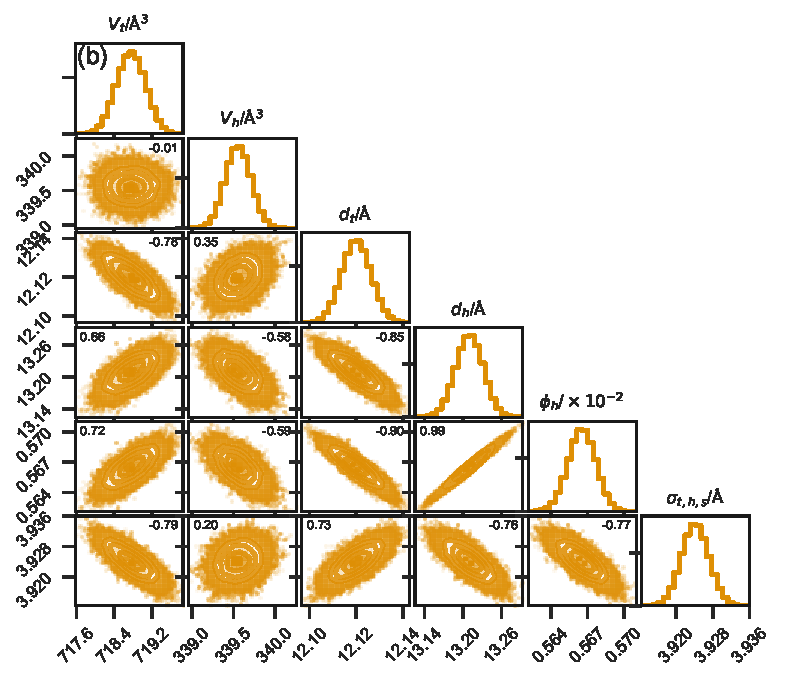
\includegraphics[width=0.49\textwidth]{reflectometry1/dmpc_xray_sp_25_pdf} \\
    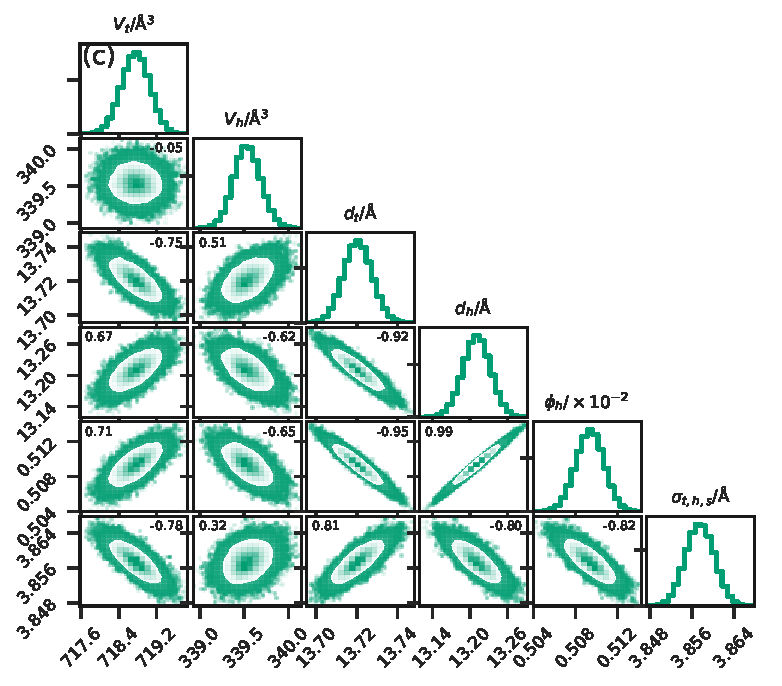
\includegraphics[width=0.49\textwidth]{reflectometry1/dmpc_xray_sp_30_pdf}
    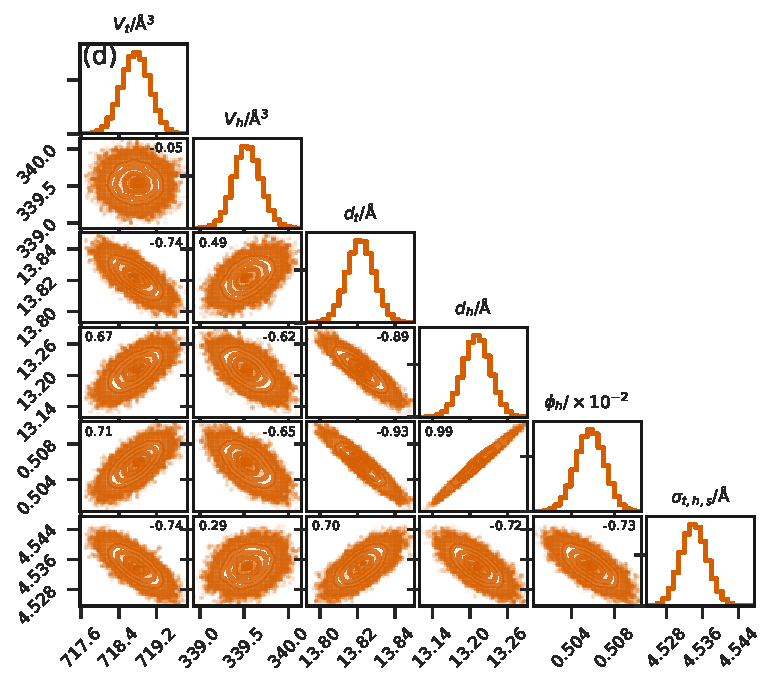
\includegraphics[width=0.49\textwidth]{reflectometry1/dmpc_xray_sp_40_pdf}
    \caption{The probability distribution functions from the chemically-consistent modelling of DMPC; (a) at \SI{20}{\milli\newton\per\meter}, (b) at \SI{25}{\milli\newton\per\meter}, (c) at \SI{30}{\milli\newton\per\meter}, (d) at \SI{40}{\milli\newton\per\meter}. The Pearson correlation coefficient for each pair of parameters is given in the top corner of each two-dimensional PDF.}
    \label{fig:dmpcpdfs}
\end{figure}
%
%
\begin{figure}
    \centering
    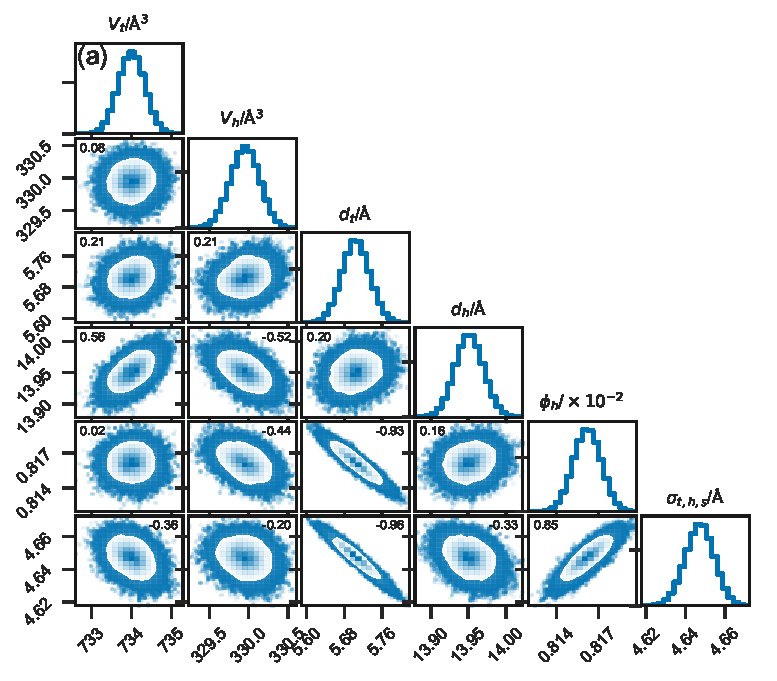
\includegraphics[width=0.49\textwidth]{reflectometry1/dmpg_xray_sp_15_pdf}
    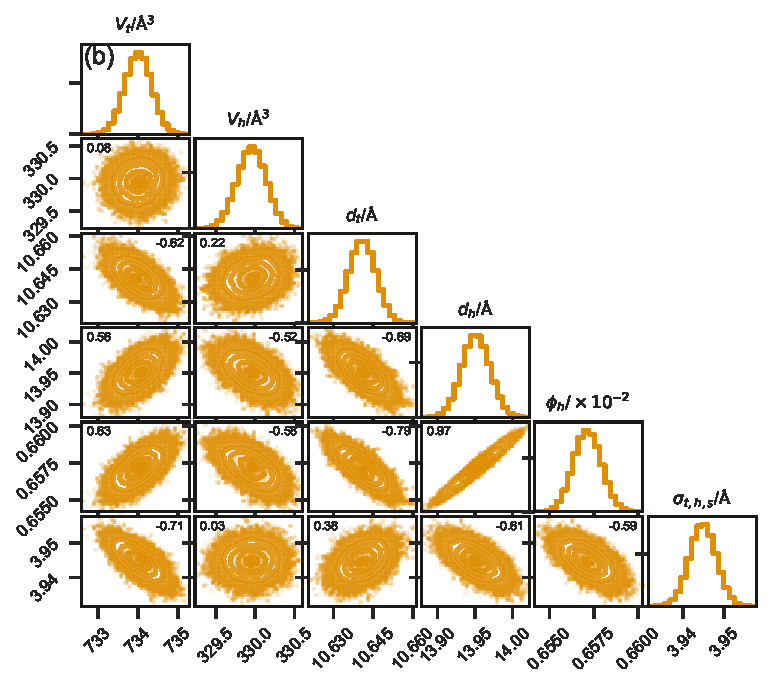
\includegraphics[width=0.49\textwidth]{reflectometry1/dmpg_xray_sp_20_pdf} \\
    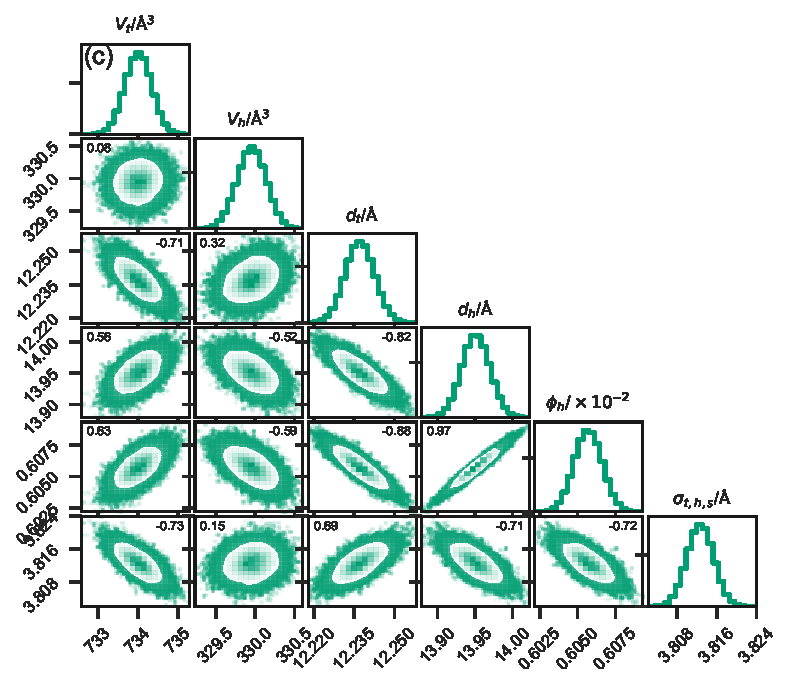
\includegraphics[width=0.49\textwidth]{reflectometry1/dmpg_xray_sp_25_pdf}
    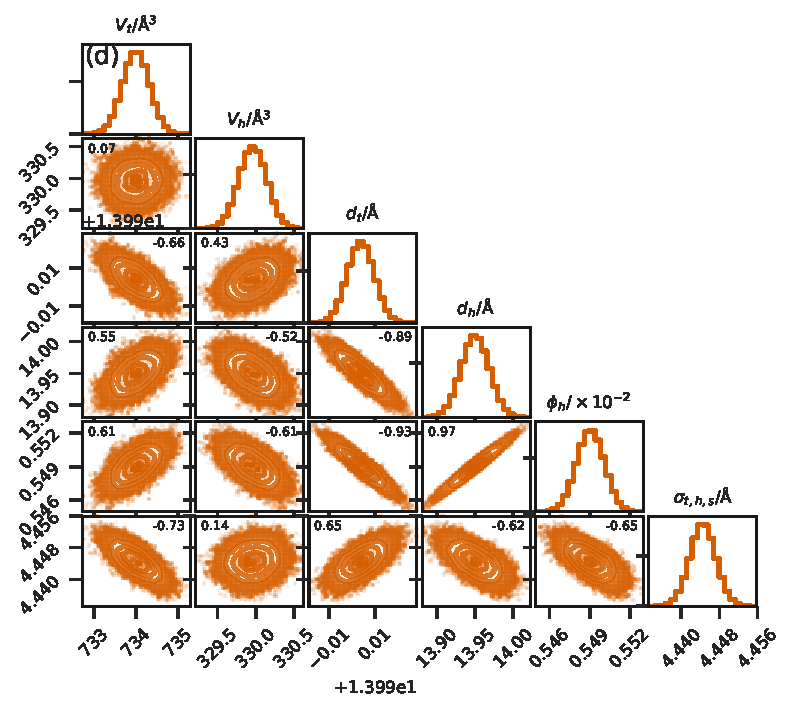
\includegraphics[width=0.49\textwidth]{reflectometry1/dmpg_xray_sp_30_pdf}
    \caption{The probability distribution functions from the chemically-consistent modelling of DMPG; (a) at \SI{15}{\milli\newton\per\meter}, (b) at \SI{20}{\milli\newton\per\meter}, (c) at \SI{25}{\milli\newton\per\meter}, (d) at \SI{30}{\milli\newton\per\meter}. The Pearson correlation coefficient for each pair of parameters is given in the top corner of each two-dimensional PDF.}
    \label{fig:dmpgpdfs}
\end{figure}
%
%
\begin{figure}
    \centering
    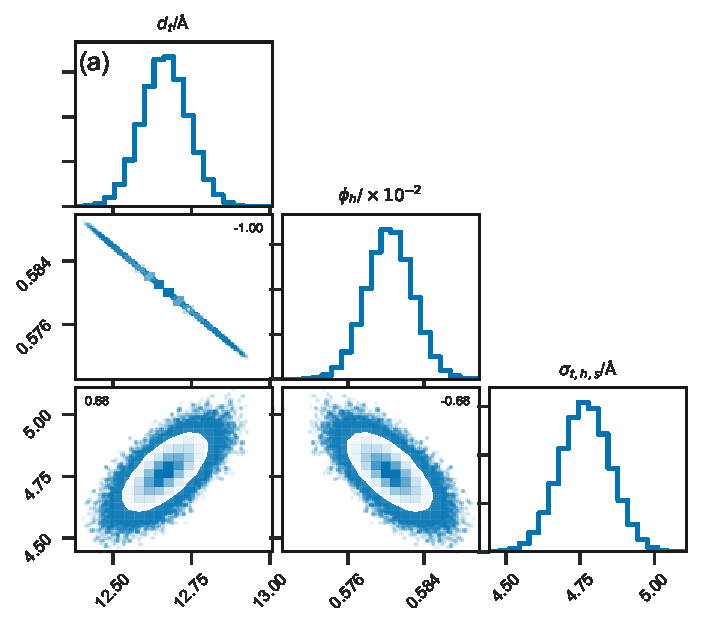
\includegraphics[width=0.49\textwidth]{reflectometry1/dppc_neutron_15_pdf}
    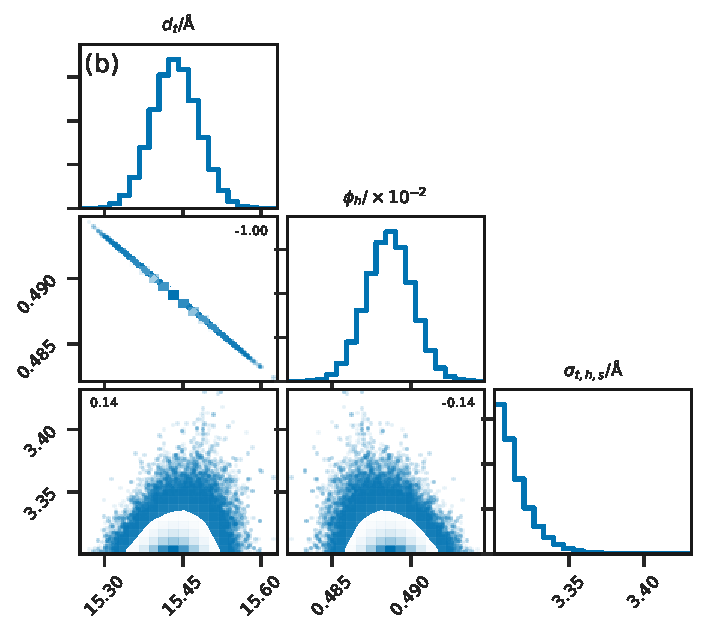
\includegraphics[width=0.49\textwidth]{reflectometry1/dppc_neutron_20_pdf} \\
    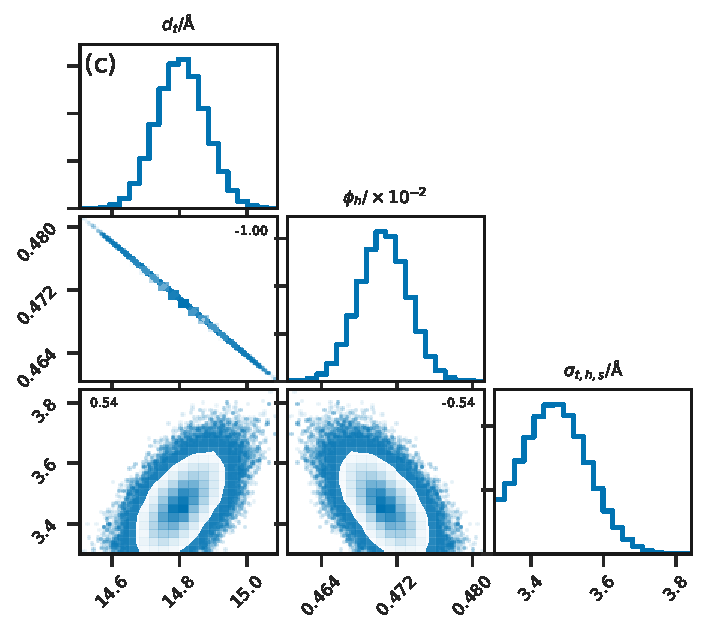
\includegraphics[width=0.49\textwidth]{reflectometry1/dmpc_neutron_20_pdf}
    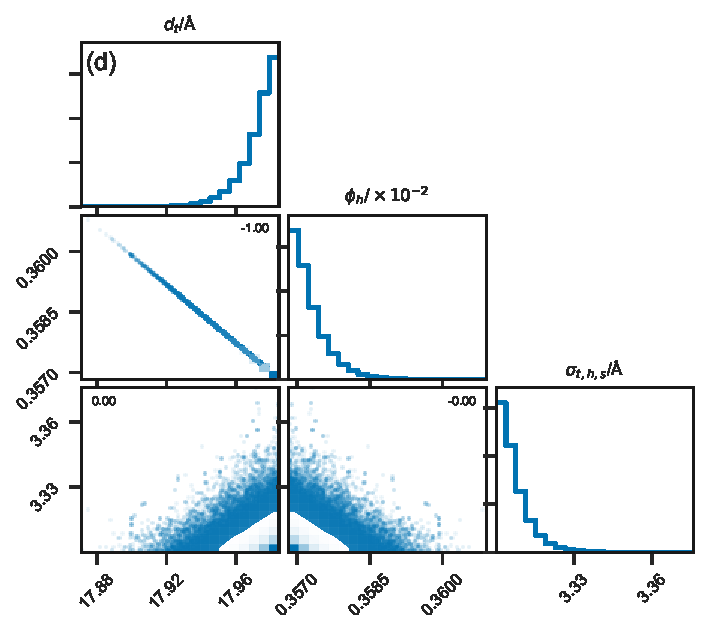
\includegraphics[width=0.49\textwidth]{reflectometry1/dmpc_neutron_25_pdf}
    \caption{The probability distribution functions from the chemically-consistent modelling of the NR data; (a) DPPC at \SI{15}{\milli\newton\per\meter}, (b) DPPC at \SI{20}{\milli\newton\per\meter}, (c) DMPC at \SI{20}{\milli\newton\per\meter}, and (d) DMPC at \SI{25}{\milli\newton\per\meter}. The Pearson correlation coefficient for each pair of parameters is given in the top corner of each two-dimensional PDF.}
    \label{fig:nrpdfs}
\end{figure}
%
